
\subsection{Robot Unit}

The robot unit consists of three assemblies: a base, a robot and a gripper (Figure \ref{fig:kr1410}).

\begin{figure}[h]
    \centering
    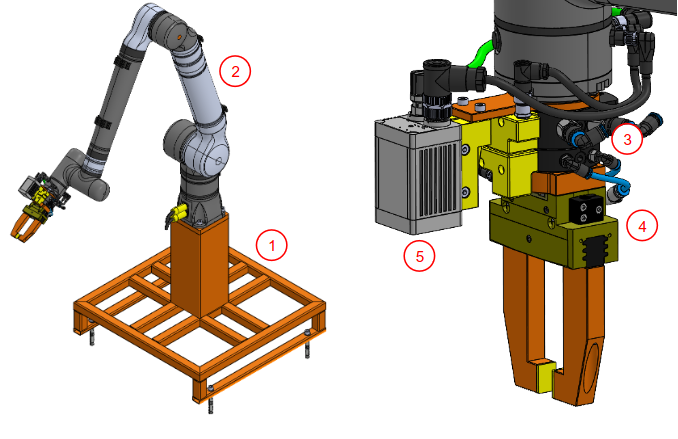
\includegraphics[width=\textwidth]{3. System Design/3.2 Hardware Selection/kr1410.png}
    \caption{Components of the robot unit: 1) robot base; 2) robot from kassow robots; 3) manual quick-change system; 4) pneumatic parellel gripper; 5) camera system}
    \label{fig:kr1410}
\end{figure}

The base is a simple welded construction made of steel. The choice of steel material ensures that the base has
sufficient dead weight so that it can be transported together with the robot and gripper using a pallet
truck without the risk of tipping over. During operation, the robot unit is fixed to the floor with four M12
screws. The robot used is a 7-axis robot from Kassow Robots. This fulfills the requirements defined in
the first work packages. The gripper is a pneumatic parallel gripper with a manual quick-change
system. The gripper was selected according to payload, gripping force and opening width. The
opening width is the dominant selection criterion here, as the gripper must be able to grip both the thin
sheets with thicknesses of around 1 to 3 mm and the handle on the drawers with a width of 15 mm. An
electric gripper was also considered, as the power supply could have been provided via the cable
already integrated in the robot. Due to the higher costs, the double height and the weight, a pneumatic
gripper was chosen.



The manual quick-change system makes it possible to exchange different gripper
designs in a short time and without increased effort if required for a sheet metal part type. Sheet metal
part is folded into something like a box. For this, it is technically sensible or necessary to use a
vacuum gripper.
This means that collision-free gripping is not possible with a parallel gripper after the last bend. The
quick-change system also has an electric and pneumatic power feed-through, which ensures simple,
user-friendly changeover.



Furthermore, a camera system is installed on the robot itself. This is used to determine the relative
position between the robot unit and the sheet pickup station, bending machine and storage shelf using the markers
and between the robot unit and the sheet metal part (when it is first made available at the
sheet pickup station or is gripped) using features on the sheet metal part.